
\section{Deriving a Corresponding Deferrable Task Set and Schedulability Test}
\label{sec:convert}

The example in Section~\ref{sec:unschedulable} can be easily converted to a corresponding deferrable task set, as explained at the end of Section~\ref{sec:unschedulable}.  Due to Theorem 5 in~\cite{Raj:suspension1991}, the feasibility of the schedule by the period enforcer algorithm depends on whether the corresponding deferrable task set can be feasibly scheduled. Therefore, before applying the period enforcer algorithm to handle segmented self-suspending sporadic tasks, we need to first derive the corresponding deferrable task set and perform the schedulability test for the deferrable task set. To reduce the pessimism of the transformation to the corresponding deferrable task set, it would be the best to have a precise transformation and an exact schedulability test. Furthermore, as demonstrated with the example shown in Figure~\ref{fig:example}, even if the conversion is done precisely, the transformed single-segment deferrable task set can admit more pessimism than the original self-suspending task set with respect to schedulability.


With the above discussions, we need to answer two questions before adopting the period enforcer algorithm. First, how can we derive the corresponding deferrable task set efficiently? Second, how should we perform the schedulability test on the corresponding deferrable task set correctly?

\subsection{Task Set Transformation}
\label{sec:transformation-exponential}

The transformation from a segmented self-suspending task set to a corresponding deferrable task set was not discussed in \cite{Raj:suspension1991}. However, in our opinion, in general, such a transformation is not an easy problem. We demonstrate the inherent difficulty by focusing on a special case and by applying the recent result provided by Nelissen et al. \cite{ecrts15nelissen}, which analyzed the exact worst-case response time for segmented self-suspending sporadic tasks with exponential time complexity. The worst-case response time analysis in \cite{ecrts15nelissen} is exact under the following conditions: 1) the task set has only one segmented self-suspending task, 2) the self-suspending task is the lowest-priority task, 3) the scheduling policy is preemptive fixed-priority scheduling, and 4) $D_i \leq T_i$ for all task $\tau_i$ in the task system.

Suppose that the system has $k-1$ regular sporadic tasks and only one segmented self-suspending task $\tau_k$. The implicit deadline of a task is equal to its minimum inter-arrival time. Suppose that task $\tau_k$ has $m_k$ segments with $m_k \geq 3$.  Converting a computation segment into a deferrable task requires deriving the worst-case deferrable time (release jitter), denoted as $\rho_k^j$, for the $j^{\mathrm{th}}$ computation segment of task $\tau_k$. Formally, if a job of task $\tau_k$ arrives at time $t$, it is guaranteed that the $j^{\mathrm{th}}$ computation segment of this job will arrive no later than $t+\rho_k^j$. Suppose that the worst-case response time of the $j^{\mathrm{th}}$ computation segment of task $\tau_k$ is $W_k^j$. Therefore,  if we can derive the exact $W_k^j$ for $j=1,2,\ldots,m_k-1$ for task $\tau_k$ in this special case, we can clearly conclude that $\rho_k^1=0$ and $\rho_k^j = W_k^{j-1}+S_k^{j-1}$ for $j=2,3,\ldots,m_k$.


Based on these considerations, it appears that, at least for the simple example, the problem is basically identical to the worst-case response time analysis of segmented self-suspending task systems. Deriving the exact $W_k^j$ for $j=1,2,\ldots,m_k-1$ for task $\tau_k$ is not an easy problem.  The method recently provided by Nelissen et al. \cite{ecrts15nelissen} can be used for this specific case to derive the exact $W_k^j$ if we assume that task $\tau_k$ has only the first $j$ computation segments and $j-1$ self-suspension intervals.  However, Nelissen et al. \cite{ecrts15nelissen} also showed that calculating the worst-case response time in the above ``simple'' case is already a very challenging problem, in which calculating $W_k^j$ would need exponential time complexity if $j \geq 2$.
In particular, Nelissen et al. \cite{ecrts15nelissen} identified several misconceptions in prior analyses, and after correcting those misconceptions, observed that deriving the worst-case response time of a computation segment in pseudo-polynomial time seems to be a very challenging problem. 

In the context of the period enforcer, we consequently observe that the only existing solution for deriving the \emph{precise} bound $W_k^{j}$ (and hence $\rho_k^j$), due to Nelissen et al.\ \cite{ecrts15nelissen},  has exponential time complexity (even for the special case above).
However, finding a safe upper bound of $W_k^j$ for $j=1,2,\ldots,m_k-1$ for task $\tau_k$ can be done in pseudo-polynomial time \cite{PH:rtss98}, if over-approximations can be tolerated. 


\subsection{Schedulability Test for A Corresponding Deferrable Task Set}
\label{sec:schedulability-test-deferrable}

Here, we explain the potential schedulability test that can be used for a corresponding deferrable task set. It may be seemingly correct at beginning that we do not have to consider the interference from the other deferrable tasks created from one segmented self-suspending task. For example, in the special task set considered in Section~\ref{sec:transformation-exponential}, one may argue that it is not necessary to consider the interference from the other computation segments of task $\tau_k$ while analyzing the feasibility of the last computation segment. However, this statement is incorrect.

Consider a task system consisting of $2$ tasks. Let $\tau_1$ denote a sporadic task without self-suspensions and parameters $C_1 = 2$ and $T_1=D_1=10$, and let $\tau_2$ denote a self-suspending task consisting of three segments with parameters  $C_2^1 = 1$,  $S_2^1 = 6$, $C_2^2=1$, $S_2^2=8$, $C_2^3=1$, and $ T_2=D_2=21$. That is, this task set is pretty similar to the task set used in Section~\ref{sec:unschedulable}. One additional computation
segment is created to illustrate the potential concerns. This task set is schedulable by fixed-priority preemptive scheduling without any enforcement since the worst-case response time of the second computation segment is $10$ and the third computation segment will suffer from the interference by at most one job from task $\tau_1$. Moreover, by using the analysis in Section~\ref{sec:transformation-exponential}, we can conclude that
\begin{equation*}
  \rho_2^1 = 0, \rho_2^2 = 9, \rho_2^3 = 18.
\end{equation*}
If we do not consider the interference from the first two computation segments of task $\tau_2$, we can conclude that the last computation segment of task $\tau_2$ has worst-case deferrable time (release jitter) $18$ and the worst-case response time of a job of task $\tau_2$ is hence $18+C_1+C_2^3=21$.

However, the above statement is not correct. Let us consider this task set under control of the period enforcer algorithm, as defined in Section \ref{sec:pe}.
Figure \ref{fig:example-deferrable-incompatible} shows the resulting schedule for a periodic release pattern. This changes the schedule of the second job of task $\tau_2$. 
The second job of task $\tau_2$ (which is released at time $21$) is affected by period enforcement. The first segment of the second job arrives at time $a^1_{2,2} = 21$, is interfered for one time unit, and suspends at time $23$. The  second segment of the second job hence resumes only at time $a^2_{2,2} = 29$. Thus, we have
\begin{align*}
	ET_{2,2}^1 & = \max\left(0 + 21,\ \mathit{busy}(\tau_2, 21)\right) = 21  \text{ and }
\\
	ET_{2,2}^2 & = \max\left(9 + 21,\ \mathit{busy}(\tau_2, 29\right) ) = 30.
\end{align*}
According to the rules of the period enforcer algorithm, the processor therefore remains idle at time $29$ because the segment is not eligible to execute until time $ET_{2,2}^2 = 30$. However, at time $30$, the fourth job of $\tau_1$ is released. As a result, the second job of $\tau_2$ suffers from additional interference and misses its deadline at time $42$.

If we further allow task $\tau_1$ to be released sporadically, the fifth job of task $\tau_1$ can be released at time $41$ instead of time $40$ in Figure~\ref{fig:example-deferrable-incompatible}. For such a case, the response time of the second job of task $\tau_2$ is $23$. This means that the worst-case response time of the deferrable task created to represent the third computation segment of task $\tau_2$ must be at least $23-\rho_2^3=5$, which equals to $C_1 + C_2^1+C_2^2+C_2^3$.

Therefore, for this specific example, we know that the schedulability test for the  corresponding deferrable task set has also to be pessimistic enough to consider the interferences from all the computation segments.

\begin{figure}[t]
  \centering  
  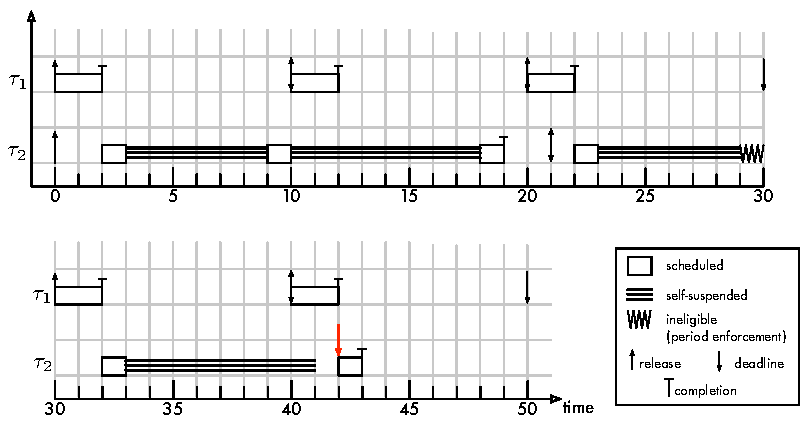
\includegraphics[scale=1]{../figures/deferrable-incompatible/deferrable-incompatible.pdf}
  \caption{}
  \label{fig:example-deferrable-incompatible}
\end{figure}

\subsection{Discussions}
\label{sec:discussions-deferrable}

The transformation from a segmented self-suspending task set to a corresponding deferrable task set and the corresponding schedulability test were not discussed in \cite{Raj:suspension1991}. With the above discussions in Section~\ref{sec:transformation-exponential} and Section~\ref{sec:schedulability-test-deferrable}, we find that the transformation is in fact non-trivial and the schedulability test of the corresponding deferrable task set has also to be pessimistic. As shown in Section~\ref{sec:schedulability-test-deferrable}, even if we derive the precise deferrable time (release jitter) information, we may still have to account for the computation segments that have no \emph{direct} interference with a computation segment that is under analysis (e.g., the third computation segment of task $\tau_2$ in Section~\ref{sec:schedulability-test-deferrable}).

Fundamentally, the design of the period enforcer algorithm relies on the schedulability of a deferrable task set. However, as we demonstrated here, there is a gap between the segmented self-suspending task set and the corresponding deferrable task set in the transformation and also in the schedulability test analysis. The authors in this paper do not find any simple way to provide a schedulability test without any information loss.

%%% Local Variables:
%%% mode: latex
%%% TeX-master: "LITES/LITES-Paper.tex"
%%% End:
